\begin{frame}
    \frametitle{Phasenfluid und kanonische Transformation}
    Zu sehen ist also
    \begin{itemize}
        \item Das Phasenfluid wird durch die Hamilton-Gleichungen beschrieben
        \item Zwei Zustände des Phasenfluid können durch kanonische Transformation in Bezug gebracht werden
        \item Für infinitessimal kleine Zustandsübergänge ist die Transformation explizit gegeben
        \item \emph{Die Bewegung des Phasenfluids ist eine stetige Abfolge kanonischer Transformationen}
    \end{itemize}
    
    \begin{displaymath}
        S(q_i,\ldots,q_n;Q_1,\ldots,Q_n;t), \quad t>0
    \end{displaymath}
    
\end{frame}

\begin{frame}
    Bisher:
    \begin{itemize}
        \item Wahl beliebiger generierender Funktion $S$
        \item Damit erhielten wir $B = -H$
    \end{itemize}
    \vspace{1cm}
    Nun Rückwärts:
    \begin{itemize}
        \item Hamilton-Funktion $H$ ist zu physikalischem Problem gegeben
        \item \begin{displaymath} -H = B = \frac{\partial S}{\partial t} \end{displaymath}
        \item Finde $S$
    \end{itemize}
    
\end{frame}


\begin{frame}
    Zu lösen ist also die partielle Differenzialgleichung

    \begin{displaymath}
        \frac{\partial S}{\partial t} + H = 0
    \end{displaymath} \\
        \vspace{1cm}
    $\longrightarrow$ Haben wir damit nicht wieder dasselbe Problem wie zu Beginn? 
\end{frame}

\begin{frame}
    Nicht ganz: \\
            \vspace{1cm}
    Hamilton findet eine Funktion, die diese Gleichung löst und damit ermöglicht, die kanonische Transformation explizit anzugeben:    
    \begin{center} \emph{Die charakteristische Funktion} \end{center}
\end{frame}

\begin{frame}
    \begin{align*}
        \text{Prinzip d. kl. Wirkung: } \quad A &= 2 \int_{\tau_1}^{\tau_2} T~dt \\
         &=  \int_{\tau_1}^{\tau_2} \sum_{i=1}^{n} p_i \dot{q}_i ~dt \\
         &= \int_{\tau_1}^{\tau_2} \sum_{i=1}^{n} p_i ~ dq_i \\[5mm]
        \text{Energieerhaltung: } \quad  H&(q_1,\ldots,q_n,p_1,\ldots,p_n) - E = 0 \\[5mm]
      \Leftrightarrow  \text{Jacobi: } \quad \min A ~ \text{ mit } ~ A &= \sqrt{2} \int_{\tau_1}^{\tau_2} \sqrt{E-V} ~ d\bar{s}
    \end{align*}
\end{frame}

\begin{frame}
  \vspace*{-0.75cm} \hspace*{-2.3cm} 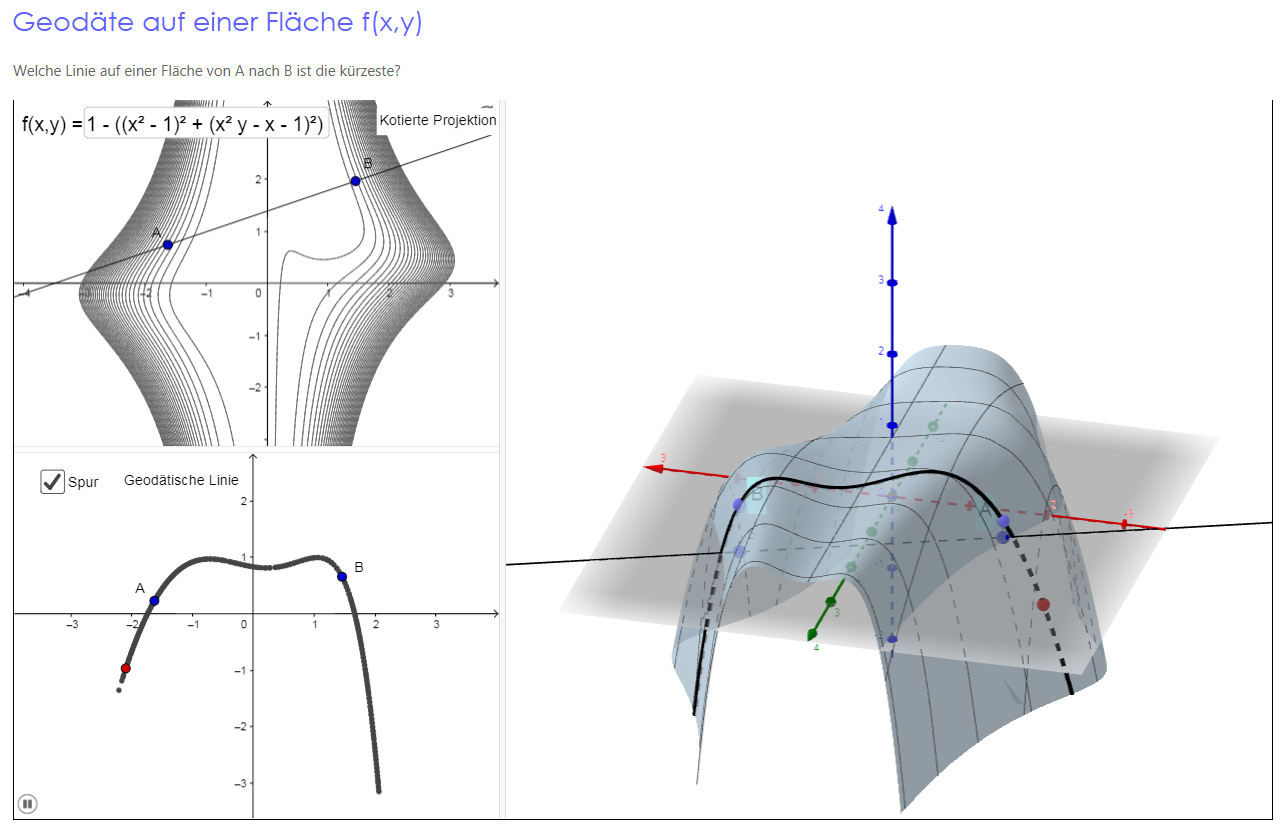
\includegraphics[scale=0.4]{images/geodaete}
\end{frame}

\begin{frame}
    \begin{itemize}
        \item Hamiltons charakteristische Funktion liefert die Länge der Geodäte zwischen Anfangs- und Endpunkt auf einer Energie-Fläche im Phasenraum
        \item Hamiltons charakteristische Funktion ist die generierende Funktion für die zugehörige kanonische Transformation
        \item Die mit Hamiltons charakteristischer Funktion generierte kanonische Transformation beschreibt die Bewegung eines Partikels im Phasenfluid
        \item $S(q_i,\ldots,q_n;Q_1,\ldots,Q_n;t)$ liefert für Anfangspunkte $Q_1,\ldots,Q_n$ für jedes $t>0$ die Lösungen $q_i(t),\ldots,q_n(t)$ der kanonischen Gleichungen 
     \end{itemize}
\end{frame}